\chapter{Inertial Waves in a Rotating Cone}

\section{Introduction}

Following the introduction and validation of the immersed boundary methods,
we now want to exemplarily investigate a rotating fluid system using these methods.
The objective is to reproduce  physical properties, with respect to theoretical and experimental results.
In relation to the research focus of the geophysical fluid mechanics research group, there are a variety
of topics of interest.\\
One area of research lies in the exploration of dynamo effects in geological and stellar systems.
In particular this means the generation of magnetic fields by electrically conducting fluids on large scales.
In this thesis we will not consider MHD-equations.  \footnote{MHD - Magnetohydrodynamic}
However in general it is considered that the helicity of a fluid domain $V$, given by

\begin{align}
    \int_{V}\dif V  \vec{v} \left( \nabla \times \vec{v} \right)
\end{align}

is directly linked to dynamo action \citep{moffat1978}.
It would be interesting to find a system which exhibits a large helicity,
as a possible candidate for future researches of the geodynamo.
Furthermore another interested is the propagation of inertial waves in different fluid domains.\\
The system we want to study in this thesis is given by a rotating cone, which is compared to
a frustum, by inserting a bottom plate into the apex.
Inertial waves are excited by a temporal modulation of the rotation frequency, which is denoted as libration.
The objective is to examine the ability to generate inertial modes or wave attractors.
Furthermore we want to study the properties of the helicity of the system and investigate the
decay of inertial oscillations.\\
In this chapter we will use linearized equations. Due to the axial symmetry with the rotating axis,
this problem could be reduced to two dimensions.
However, we want to test the code in a three dimensional setup.
One reason for this is a possible future application.
The objective would be to study the decay of turbulence in the apex of the cone.
A simulation in three dimensions can not be avoided in this case.


\section{Conventions \& Setup}
\label{cone:convsetup}

This section introduces the setup which has been used for the simulations presented in this chapter.
Fig. \ref{cone:setup_image} shows the geometry of the fluid domain.
In the remaining sections of this chapter we want to use the following conventions:

\begin{multicols}{2}
\begin{description}
    \item[$H$]{Total height of the simulation domain}
    \item[$h_c$]{Height of the cone/frustum}
    \item[$h_b$]{Height of the bottom plate}
    \item[$R$]{Radius at the top of the cone/frustum}
    \item[$r$]{Radius at the bottom  of the frustum,\\ for the cone $r=0$}
    \item[$O$]{Offset at the top of the cone/frustum}
    \item[$\alpha$]{Slope of the cone/frustum}
    \item[$\theta$]{Propagation angle of an inertial wave, with respect to the horizontal axis.}
    \item[$\Omega$]{Rotation rate}
    \item[$\omega$]{Frequency of the libration}
    \item[$\epsilon$]{Amplitude of the libration, default is 1}%\footnote{Not important due to the linearization}}
    \item[$l_x, l_y, l_z$]{Size of the total simulation domain in x, y and z direction}
    \item[Cone] {The entire cone with apex, and a possible offset at the top, this setup is obtained by setting $r=0$}
    \item[Frustum]{The cone but with a bottom plate at the bottom, hence $r>0$}
    \item[Critical Frequency $\omega_c$]{This is the libration frequency where the propagation direction of an inertial wave is parallel to the slope ($\theta=\alpha$)}
\end{description}
\end{multicols}

%For the implementation the testcase function template introduced in chapter () is used.
%The use of the different parameters with this template is shown in Appendix ().

\begin{figure}[!bp]
  \centering
        \resizebox{0.6\textwidth}{!}{
       \import{gfx/cone/conesim//}{setup.pdf_tex}
      }
      \caption{Numerical Setup for the Simulations \label{cone:setup_image} }
\end{figure}
\clearpage

\section{Theoretical Description}
\label{cone:theorie_theo}

This section gives a brief theoretical description of the problem we adapted from \citep{Greenspan1969}, \citep{Beardsley1970}.
Instead of a cone, a comparison to the two-dimensional analogy of a wedge, is made.
This system is based on the idea to introduce a geometric shape containing a singularity.\\
Let us consider the propagation of an inertial wave ray, emitted at one of the upper edges of
the wedge, as shown in Fig. \ref{cone:theorie}.
The wave propagates under the angle $\theta$, with respect to the horizontal axis.
For each reflection the propagation angle with respect to the rotation axis is preserved.
In the case of $\theta<\alpha$ we have a supercritical reflection,
thus a downward traveling wave ray is reflected downslope.
As a result the wave travels towards the lower vertex of the wedge.
It can be shown from the reflection properties, given by Eq. \ref{theorie:reflections},
that the time for a wave ray to travel the path between two reflections is constant \citep{Beardsley1970}.
To be more precise
\begin{figure}[!bp]
  \begin{minipage}[c]{0.6\textwidth}
      \centering
        \resizebox{0.7\textwidth}{!}{
       \import{gfx/cone//}{cone.pdf_tex}
      }
  \end{minipage}
  \begin{minipage}[c]{0.3\textwidth}
      \caption{
          Propagation of an inertial wave emitted from the top edge of a wedge,
           where $\theta$ indicates the direction parallel to the group velocity
            $\vec{c_g}$.  $L$ and $L^{\prime}$ are the path lengths before and after a reflection.
      \label{cone:theorie}
      }
  \end{minipage}
\end{figure}


\begin{align}
    \frac{L}{|\vec{c}_g|} = \frac{L^{\prime}}{|\vec{c}_g^{\prime}|}
\end{align}

where $L$ is the path length between to reflections, the prime denotes the properties after a reflection.
This means that the overall propagation time into the apex of the cone becomes infinity, along with the energy density and the wave number.
Thus, the apex is acting as an attractor to inertial waves.
As a conclusion it follows that since no reflection out of the cone apex can occur, the possibility of inertial modes is not given.

\section{Experiment}
\label{cone:theorie_exp}

For a test of these theoretical assumptions, an experimental study was performed by \citep{Beardsley1970}.
The schematic setup is shown in Fig. \ref{cone:setup_experiment}.
In the first part of the experiment, a plexiglass cylinder, containing a conical shaped cavity,
of height $H=\SI{19.95}{\centi\meter}$ and a radius of $r=\SI{8.91}{\centi\meter}$ was used and filled with water.
The apex half angle was set to $\beta=24^{\circ}3.7^{\prime}$ degree.
For the rotation rate a frequency of $\Omega_0 =\SI{6.28}{\radian\per\second}$ was chosen.
The resulting Ekman number is

\begin{align}
    \Ekman = \frac{\nu}{\omega r H^2} \approx 7.72\cdot 10^{-6}
\end{align}

where $\nu = \SI{1.0}{\milli\pascal\second}$  \citep{tipler2003}.
In order to exite inertial waves the cone is librating.
The total rotation rate is proportional to

\begin{align}
\Omega(t) = \Omega_0 + \epsilon_0 \omega \cos(\omega t)
\end{align}

where $\omega$ is the libration frequency with the amplitude $\epsilon_0=\SI{0.2}{\radian}$.
The excitation of the fluid results from the wall friction, induced
by the modulation of the constant rotation frequency $\Omega_0$.

\begin{figure}[!b]
      \centering
        \resizebox{0.6\textwidth}{!}{
       \import{gfx/cone///}{experiment.pdf_tex}
      }
      \caption{
          Experimental Setup. In the first experiment a cone is used (left). For the second part the apex of the cone
          is replaced by a frustum (right).
      \label{cone:setup_experiment}
      }
\end{figure}

For the analysis the dynamic pressure field was measured at different depths along the rotation axis.
The ratio of libration to the constant rotation frequency was varied in the range of ${0.25\leq\omega/2\Omega_0\leq1}$.
The pressure and phase lag spectrum  show that no consistent peaks are observable for different measurment heights.
Hence, no inertial modes are existing.
\\
In the second part of the experiment, the apex of the cone was replaced by a frustum,
with a bottom plate at the position $z/H = 0.261$.
This setup yields the possibility that a wave ray can be reflected on the bottom.
The pressure and phase lag spectrum in this setup show that
independent of measurement depth of the pressure, resonances occur which can be associated with standing waves.
Hence, inertial modes exist.
\\
\\
One objective in this thesis is to compare the simulation results to this experiment.
Some considerations regarding the experiment shall be briefly discussed here.
For our setup the relation between libration frequency $\omega$ and the propagation angle $\theta$
is given by Eq. \ref{theorie:eq_rot_dispersion}, which can be simplified to

\begin{align}
    \omega = 2\cos(\theta)
\end{align}

This means that for $\omega = 2\cos(\alpha)$ the propagation angle of an inertial wave is parallel to the slope of the cone.
Depending on the libration frequency two different motions can occur in the cone

\begin{description}
    \item[$\omega < \omega_c$]{It holds that $\theta > \alpha$. A downward traveling wave is reflected upwards on the slope of the cone}
    \item[$\omega > \omega_c$]{It holds that $\theta < \alpha$. A downward traveling wave is reflected downwards on the slope of the cone}
\end{description}

For the first case the apex of the cone will not act as an attractor.
This first scenario is not addressed directly in the experiment, in this chapter it will be investigated in more detail.

\section{Numerical Implementation of Libration}

For the numerical implementation of the experiment, a modified set of the equations
introduced in Sec. \ref{THEORIE:ROT}, is presented here.
It has to be concerned, that the system has now a time-dependent rotation rate.
For the non-dimensional system we set

\begin{align}
    \vec{\Omega}(t) = 1 \; + \; \epsilon \sin(\omega t)\vec{e}_z
\end{align}

There are two options for an implementation.
First of all, a rotating coordinate system with a constant velocity $\Omega_0$ can be chosen.
This enables the direct use of the Eqs. \ref{theorie:rotns}. Since the overall rotation rate of the system is
modulated, it is necessary to introduce the boundary conditions

\begin{align}
    \vec{v}|_{Border}  = \Omega \times \vec{r} = \begin{pmatrix}
           -y ( 1 + \epsilon \sin(\omega t)) \\
            x ( 1 + \epsilon \sin(\omega t)) \\
           0\\
         \end{pmatrix}
\end{align}

However, obtaining a linearized version of the boundary methods is not as easy.
In addition it can be assumed that it is safer to use No-Slip boundaries with zero velocity, as
the taylor-couette system showed that velocities other than zero can create a larger numerical error.
The alternative option is the introduction of an accelerated frame of reference.
In this case the boundary conditions do not need to be modified, but the coriolis forcing term $\vec{f}$ is given by \citep{Tilgner2007}.

\begin{align}
    \vec{f} &= 2 \vec{\Omega} \times \vec{v} + \pdn[]{t}\left(\vec{\Omega} \times \vec{v} \right)
            = \begin{pmatrix}
           -y \omega \epsilon \cos(\omega t) \\
           -x \omega \epsilon \cos(\omega t) \\
           0\\
         \end{pmatrix}
            + 2\begin{pmatrix}
           - ( 1 + \epsilon \sin(\omega t)v_x \\
             ( 1 + \epsilon \sin(\omega t)v_y \\
           0\\
         \end{pmatrix}
            = \begin{pmatrix}
           -y \epsilon \cos(\omega t) \\
           -x \epsilon \cos(\omega t) \\
           0\\
         \end{pmatrix}
\end{align}

In the last step the linearization was introduced.
The non-linear advection term is removed from the equations of motion, which
are then given by

\begin{align}
    \label{cone_theorie:rotns}
    \pdn[v]{t} = -c^2\nabla \rho + \Ekman \Delta \vec{v} + \vec{f} \qquad;& \qquad  \nabla \vec{v} = 0
\end{align}

Finally, one additional stability criterion shall be introduced.
It is important that the time for propagating information from on side of the domain
to the other is much smaller than the overall rotation rate.
\footnote{Private communication with A. Tilgner}
This can be estimated by

\begin{align}
    t = \sqrt{\frac{2}{c^2}} << 2\pi
\end{align}

where $c$ is the artificial speed of sound.
Thus the propagation time and therefore this criterion, depends on the artificial sound speed $c$.
A good estimation is given by setting $c^2 = 500$.
It could be observed that otherwise, not only physical wrong results are obtained but also
numerical instabilities can occur.
\footnote{Private communication with O. Goepfert}

\newpage

\section{Data Analysis}

The main interest, in the analysis of the simulation data, lies in the identification of possible inertial modes.
An appropriate choice is to consider the energy in the $z$-component of the  velocity, which is given by

\begin{align}
    \left<v_z^2 \right>(t) =  \int \dif V v_z(t)^2 \approx \sum_{i, j, k}^{N_x,N_y,N_z} \Delta x \Delta y \Delta z \left.v_z(t)^2 \right|_{i,j,k}
\end{align}

This has multiple benefits

\begin{itemize}
    \item The $v_z$-velocity component is independent of the coordinate system which is used, it is not necessary
                to compute a transformation to inertial frame.
    \item The energy induced by the libration is perpendicular to this component, thus all components
            in the $v_z$-component are created by inertial oscillations.
\end{itemize}

In Fig. \ref{fig:cone:cyl_vzmode}, this energy is shown exemplarily for two libration frequencies for a cylinder.
\footnote{The results are taken from Sec. \ref{cone:sec:lib_cylinder}}
For a resonance of the system ($\omega=1.2$), it takes further time until a steady state, with a constant oscillation is reached.

\begin{figure}[!pb]
  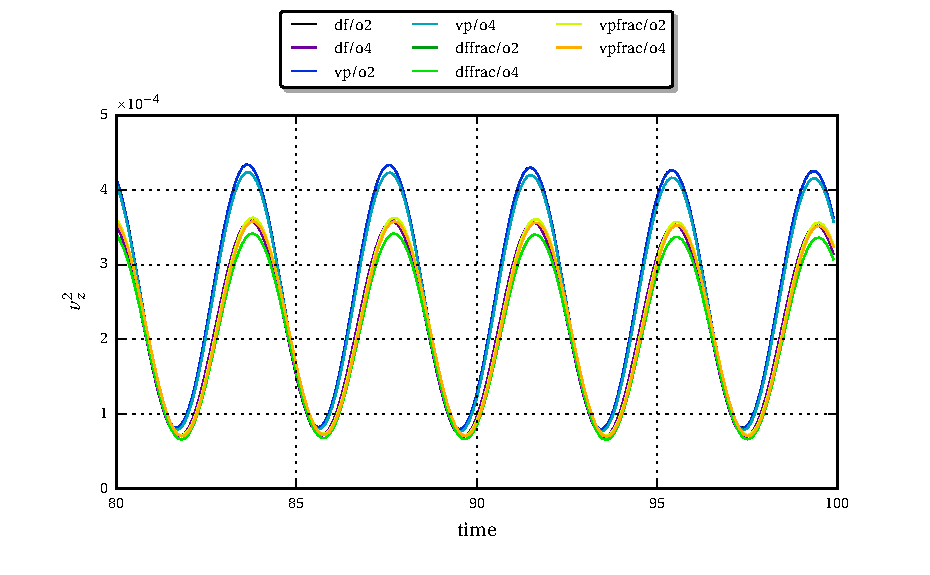
\includegraphics{gfx/cone/cylinder/cyl_vz.pdf}
  \caption{Kinetic energy in $z$-direction for the Direct-Forcing method of 2nd order, at different libration frequencies.
  \label{fig:cone:cyl_vzmode}
  }
\end{figure}
\clearpage

In order to obtain a spectrum, the energy amplitude is taken from the last two extrema of $<v_z^2>$.
The computation is given by

\begin{align}
    A\left(\left<v_z^2\right>\right) = \frac{\max(\argmax(\left<v_z^2\right>_{v})) - \max(\argmin(\left<v_z^2\right>_{v}))}{2}
\end{align}

Since the error of this calculation depends on the total simulation time, it was ensured that all simulations
were carried out long enough.
For the same simulation times, the error of one resonance is estimated in the range $\sigma_A \approx 5\% - 10\%$,
When no resonances are present, the error is estimated to be of order $\sigma_A \approx 2.5\% - 5\%$.\\
Another part of the analysis is the computation of the relative helicity of the system, given by \citep{PAPER}.

\begin{align}
H(t) = \frac{\int_V \dif V \vec{v} (\nabla \times \vec{v})}
{\int_V \dif V |\vec{v}| \int_V \dif V |\nabla \times \vec{v}|}
 = \frac{\sum_{i,j,k=0}^{N_x, N_y, N_z} \vec{v}_{i,j,k} (\nabla \times \vec{v}_{i, j, k})}
 {\left(\sum_{i,j,k=0}^{N_x, N_y, N_z}|\vec{v}_{i,j,k}|\right)
 \left(\sum_{i,j,k=0}^{N_x, N_y, N_z}
 | \nabla \times \vec{v}_{i, j, k}|\right)}
\end{align}

For the discretization of the rotation operator, a central difference scheme of 2nd order is used.
\clearpage

%%%%%%%%%%%%%%%%%%%%%%%%%%%%%%%%%%%%%%%%%%%%%%%%%%%%%
%%%%%%%%%%%%%%%%%%%%%%%%%%%%%%%%%%%%%%%%%%%%%%%%%%%%%
%%%% CYLINDER
%%%%%%%%%%%%%%%%%%%%%%%%%%%%%%%%%%%%%%%%%%%%%%%%%%%%%
%%%%%%%%%%%%%%%%%%%%%%%%%%%%%%%%%%%%%%%%%%%%%%%%%%%%%


\section{Simulation of a Librating Cylinder}
\subsection{Introduction}
\label{cone:sec:lib_cylinder}

As a first step towards the implementation of the librating cone, simulations of fluid flow in a librating cylinder were carried out.
Despite the theoretical and experimental results we discussed so far,
it is difficult to find results in literature which would be suitable for an appropriate validation for the cone.
For the cylinder on the other hand, theoretical and numerical results are available \citep{Greenspan1990}, \citep{Sauret2012}.\\
The theoretical solution for the inviscid case was introduced in Sec. \ref{theorie:rotating:cyl_modes}.
Due to the excitation by libration the possible observable modes have to be axially symmetric, meaning the azimuthal wavenumber is zero.
All possible modes are therefore defined by the indices $(n, m)$, corresponding to the radial and axial wavenumber.\\
The simulations were performed with a librating cylinder, of aspect ratio $\Gamma=r/H=\nicefrac{0.5}{1.1}$
\footnote{Due to a misunderstanding the aspect ratio of the cylinder was set to $\Gamma=r/H=\nicefrac{0.5}{1.1}$ instead of $\frac{1}{2}$.}
, and a varying libration frequency.
The main simulation parameters are given by


\begin{center}
\vspace*{0.7ex}
\begin{tabular}{c|c|c|c|c|c|c|c }
 $\omega $ & $\Gamma$ & $\Delta t$ & $\Delta x$ & $c^2$ & $\Ekman$  & $l_x, l_y, l_z$ & $T_{end}$\\
\hline
 $[0.2,\; 2], \Delta \omega = \nicefrac{1}{10}$ & $\nicefrac{0.5}{1.1}$ & $10^{-4}$ & $\nicefrac{1}{128}$ & 500 & $10^{-4}$  & (1.1, 1, 1) & 100\\
\end{tabular}
\vspace*{0.7ex}
\end{center}

The simulations were performed for all immersed boundary methods used in this thesis, with 2nd and 4th order finite difference schemes.
The results are presented and discussed separately in comparison to the results of the librating cone in the next section, for reasons of clarity.

\clearpage


\subsection{Results}
\subsubsection{Frequency Spectrum}

For all simulations, the kinetic energy of the $z$-component of the velocity was computed.
The results for the computation of the amplitude $A\left(\left<v_z^3\right>\right)$, in dependcy of the libration
frequency are shown in Fig. \ref{fig:cone:cyl}.
All immersed boundary methods show a similar profile.
The largest amplitude deviations can be spotted at a frequency of $\omega=1.2$ and are about $5\cdot10^{-3}$.\\
It can be noted that at this position the largest resonance M\RN{1} occurs which is about $3.5\cdot10^{-2}$.
Two other resonances can be observed at $\omega=0.75$ (M\RN{2}) and $\omega\approx1.7$ (M\RN{2}), which are
about ${\approx1.3\cdot10^{-2}}$.
To make the deviations between the methods more visible, two inset plots which are
set to the location $\omega=0.8$ and $\omega=1.0$., are shown.
For both positions, the largest amplitude is given by the Direct-Forcing method of 2nd order, followed by
the Volume-Penalization method of 2nd and 4th order.
The amplitude difference between the first two methods is just slightly visible when looking at the right inset plot.
It seems like these three methods yield nearly the same results for all frequencies.
For all remaining methods  no strict order or grouping can be recognized.\\
The results for the interpolation method are not presented here, since the simulations became numerically unstable.

\subsubsection{Eigenvalues for the inviscid equations}

For a comparison to the theoretical solution, the eigenvalues for the (n, m)-inertial modes with $n\in[1,6]$ and $m\in[1, 2]$ were computed.
The results are shown in Table \ref{cone_cyleigenvalues}.
There are four possible candidates,  which could correspond to the peaks in the spectrum.
The largest peak at M\RN{1} is close to the eigenvalues of the (2, 1) and (4, 2) mode.
The left peak  M\RN{2} could be related to the (2, 2) mode,  whereas the peak on the right side M\RN{3} is close to the eigenvalue of the (4, 1) mode.
The eigenvalues for uneven $n$ are not considered. Due to the excitation by libration,  only azimuthal velocity fields which are even,
in relation to the plane $z=H/2$ are possible \citep{Sauret2012}.
\footnote{An uneven pressure gradient from the theoretical solution results in an even velocity field.}
Furthermore we are not considering modes with $m\geq2$. These modes are not even visible at an Ekman number of $5\cdot10^{-5}$,
due to viscous damping of large wave numbers, according to \citep{Sauret2012}.\\
A further comparison was done by computing the eigenmodes for the possible (n, m) values of M\RN{1}, M\RN{2} and M\RN{3}.
The results are shown in Fig. \ref{cone:cyl_modes}.
The assumed (4, 2) mode is not shown since the profiles do not match.
The theoretical solution yields the pressure field of the inertial mode.
Since this quantity is not directly accessible from the simulation results,
the absolute velocity in $z$-direction, integrated over the simulation time, is computed.
This expression should be proportional to the theoretical pressure gradient in $z$-direction.
With exception of the sign, which is eliminated by taking the absolute value of $v_z$.
\clearpage
\begin{figure}[!t]
  \centering
  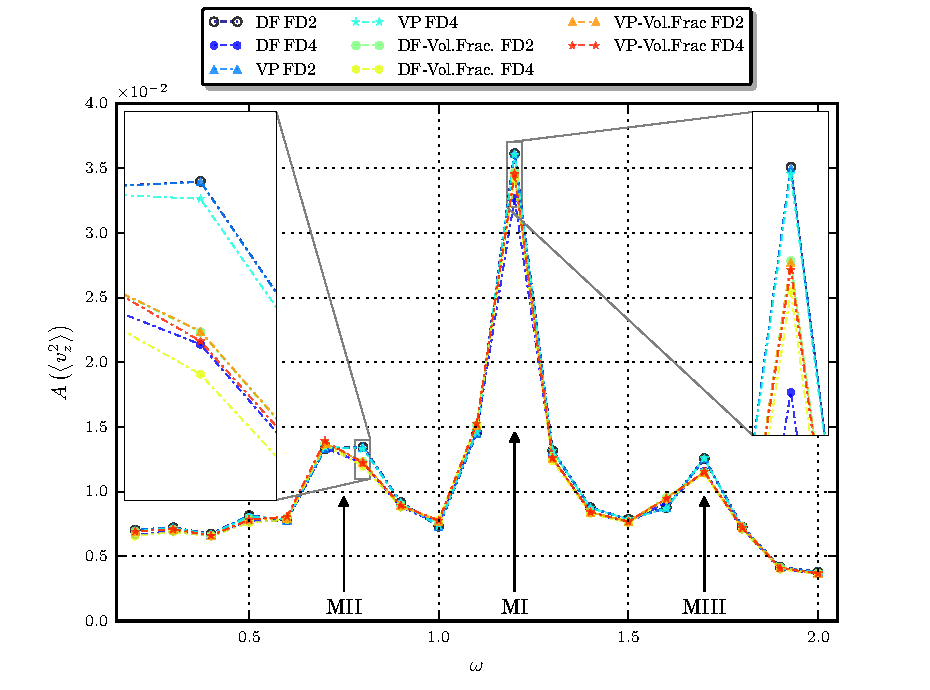
\includegraphics{gfx/cone/cylinder/cylinder.pdf}  \caption{\label{fig:cone:cyl}
    Amplitude of the kinectic energy in $v_z$, as function of the liberating frequency $\omega$.
   For the Direct-Forcing (DF), Volume-Penalization (VP) method with and without Volume-Fraction and
      2nd(o2)  and 4th(o4) order finite differences.}
\end{figure}

\bgroup\large
\begin{table}[!b]
\centering
\def\arraystretch{1.5}%
\begin{tabular}{c c c c c}\toprule
            &    m =  1  & m = 2   &    \\ \hline
\midrule
        n=1 &   0.698433         &              0.398913 &    \\
        n=2 & \cellcolor{blue!25}  1.195232         &        \cellcolor{blue!25}      0.754094 &    \\
        n=3 &   1.490715         &              1.042313 &    \\
        n=4 &  \cellcolor{blue!25} 1.660912         &     \cellcolor{blue!25}         1.262759 &    \\
        n=5 &   1.762270         &              1.426587 &    \\
        n=6 &   1.825743         &              1.547435 &    \\ \hline

\bottomrule
\end{tabular}
\caption{Eigenvalues of the (n, m)-inertial modes in a cylinder with aspect ratio $\nicefrac{5}{11}$.
            Possible modes are highlighted.  \label{cone_cyleigenvalues} }
\end{table}
\egroup
\clearpage


\begin{figure}[!t]
  \centering
  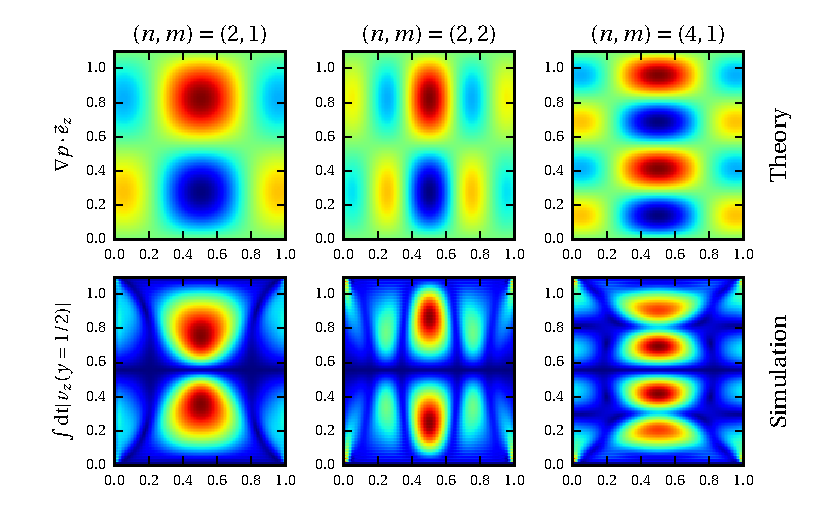
\includegraphics{gfx/cone/cylinder/modes.pdf}  \caption{
      Theoretical inertial modes compared to the absolute of the velocity component $v_z$ of the simulation.
      For the peaks \RN{1}, \RN{2} and \RN{3}.
      \label{cone:cyl_modes}}
\end{figure}

The theoretical profiles for the inviscid problem look indeed very similar to the simulated profiles.
The simulation profiles are slightly distorted on the walls of the fluid domain, in
comparison to the theoretical profiles.
For all modes, the number of wave nodes in $z$, and $x$ direction is identical,
 when comparing the theoretical and numerical profiles.

\subsubsection{Helicity}

The computation of the helicity was split into an integral over the upper and lower half
of the cylinder.  A result for $\omega=1.5$ is exemplarily shown in Fig. \ref{cone:cyl_helicity}.
In the upper half of the cylinder a negative helicity can be observed, the maximum of the amplitude is of order $10^{-1}$.
In the lower half of the cylinder a positive helicity can be observed, the maximum is of the same order.
The helicities are symmetric with respect to zero, thus $H_{\text{up.}} = -H_{\text{low.}}$.
As a result it, the total helicity of the cylinder is zero for all times.

\begin{figure}[!p]
  \centering
  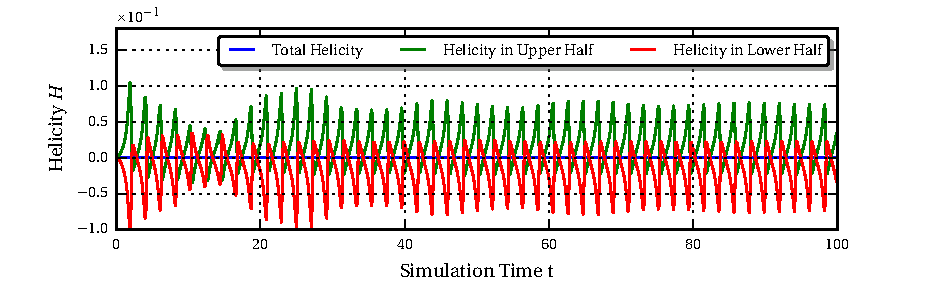
\includegraphics{gfx/cone/cylinder/helicity.pdf}  \caption{
      Time-dependent Helicity $H(t)$ for $\omega=1.5$. The Direct-Forcing method of 2nd order was used.
      \label{cone:cyl_helicity}
      }
  \centering
  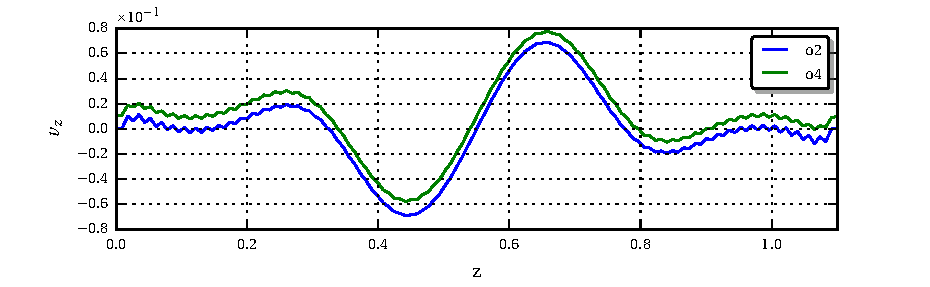
\includegraphics{gfx/cone/cylinder/oscillations.pdf}  \caption{
      Numerical oscillations along the $z$ axis trough $(x,y) = 0.5, 0.5$.
      For Direct-Forcing method of 2nd (o2) and 4th (o4) order, at $\omega=1.5$.
      \label{cone:cyl_oscillations}
      }
  \centering
  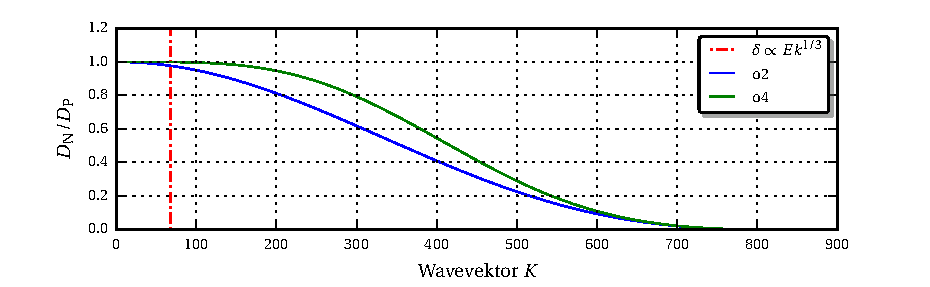
\includegraphics{gfx/cone/cylinder/numvis.pdf}  \caption{
      Ratio $D_N/D_P$ of  numerical viscosity  $D_N$ and physical viscosity computed for $\Ekman=10^{-4}$. For 2nd and 4th- order central differencing schemes.
      The red line indicates the wave number of an inertial wave with width $\Ekman^{1/3}$.
      \label{cone:cyl_numvis}
      }
\end{figure}

\subsubsection{Numerical Oscillations}

For all immersed boundary methods numerical oscillations are observable.
Fig. \ref{cone:cyl_oscillations} shows this for the Direct-forcing method of 2nd and 4th order and $\omega=1.5$.
The profile is taken along the $z$-Axis at $(x,y)=(\nicefrac{1}{2},\nicefrac{1}{2})$.
It can be noted that the error is larger in the regions near to the wall.
One important detail is that the oscillations are only observable in $z$-direction, not
in th $(x,y)$ plane.
For the 4th order method the upwind scheme has been used, in contrast to the FTCS-Scheme at 2nd order.
It is visible that the oscillations are slightly diminished, when using the 4th order scheme.

\subsubsection{Numerical Viscosity}

The ratio between the numerical and physical viscosity was computed, according to Eq. \ref{NUMERIC:NUMVIS}.
The results are shown in Fig. \ref{cone:cyl_numvis}.
The red bar denotes the wave number for the width of an inertial wave, which is $\propto \Ekman^{1/3.}$.
For this value the ratio is $\approx{0.977}$.
For both methods a decrease in the numerical viscosity can  be observed.
At larger wave numbers, the 4th order method has a better approximation than the 2nd order method.
The largest wave number of the  system is possible for $\lambda = 2\Delta x$,
it follows that $K_{\text{max}} = \nicefrac{2\pi}{\lambda} \approx 402.1$.
\clearpage

\subsection{Discussion}

\subsubsection{Frequency Spectrum}

We assume that the peaks in the frequency spectrum can be identified as inertial modes.
The computed eigenvalues  are close to the peak positions in the spectrum and a first good indicator.
However  the assumption that M\RN{1} could be the (4, 2)-Mode is wrong.
The representation of the averaged $v_z$-component in Fig. \ref{cone:cyl_modes}, in comparison to the pressure gradient
clarifies that the peak M\RN{1} corresponds to the (2, 1)-Mode.
M\RN{2} corresponds to the (2,2)- Mode and M\RN{3}  to the (4, 1)-Mode.\\
The distortion in the averaged velocity profiles can be explained by the viscous friction from domain boundaries.
The results of the simulations are therefore in a good agreement with the theoretical description of the inviscid case.
\\
A numerical study of the non-linear system was performed by \citep{Sauret2012}.
The inertial modes, which were found in this study confirm the present results.
One difference is a slight shift $\approx0.06$ of the eigenvalues,
due to the mistakenly used aspect-ratio.
Furthermore three additional modes were found in this study, which do not occur
in the frequency spectrum in this thesis.
One explanation for this the use of larger Ekman number in this simulations $\propto10^{-4}$.
The width of a resonance peak is proportional to the damping rate of the system, in analogy to an harmonic oscillator.
\footnote{Private communication A.Tilgner}
Due to the stronger damping in our simulations the spectrum shows broader resonance peaks than in the study of \citep{Sauret2012}.\\
All methods are able to reproduce these results, with exception of the interpolation method.
Unfortunately, it was not possible to figure out the reason for the numerical instability.
The almost identical errors of the Volume-Penalization and Direct-Forcing method of 2nd order
indicate that the timestep could be to small.
The velocities local to the domain boundaries are so small, that the damping force (Volume-Penalization method) is almost identical
to setting the velocity direct to zero (Direct-Forcing method).

\subsubsection{Numerical Oscillations}

The velocities in the system are at least of order $\cdot10^{-1}$. The resulting Peclet number is
given by
\begin{align}
    \Pe = \frac{0.1\cdot\nicefrac{1}{128}}{\Ekman} =15.625
\end{align}

This value gives a possible explanation for the occurence of oscillations,
since it violates the stability criterion $\Pe<2$.
The improvement from the upwind scheme support this assumption.
It still remains unclear why the oscillations only occur in the $z$-direction.
%Furthermore this is in accordanc
%Oscillations usually occur where the velocity gradient is high.
%This can also be seen from the velocity profile of the (2, 2)-mode in figure \ref{cone:cyl_modes}.
%It is possible that the gradient arises from the corners on top and botom of the cylinder
%which is at

\subsubsection{Numerical Viscosity}

The numerical viscosity was computed in order to determine its influence on the system.
For the physical properties of our system, we estimate wavelengths in the range of $1 - \Ekman^{1/3}$.
The error of the numerical viscosity in this range can be neglected.

\subsubsection{Helicity}

The computation shows that the total helicity of the cylinder is zero.
This result is not unexpected.
Due to the axial symmetry in $z$-direction, the helicities in the upper and lower part of the cylinder cancel each other.

\newpage
%%%%%%%%%%%%%%%%%%%%%%%%%%%%%%%%%%%%%%%%%%%%%%%%%%%%%%%%%%%%%%%%%%%%%%%%%%%%%%%%%%
%%%%%%%%%%%%%%%%%%%%%%%%%%%%%%%%%%%%%%%%%%%%%%%%%%%%%%%%%%%%%%%%%%%%%%%%%%%%%%%%%%
%%%%%%%%%%%%%%%%%%%%%%%%%%%%%%%%%%%%%%%%%%%%%%%%%%%%%%%%%%%%%%%%%%%%%%%%%%%%%%%%%%
%%%%%%%%%%%%%%%%%%%%%%%%%%%%%%%%%%%%%%%%%%%%%%%%%%%%%%%%%%%%%%%%%%%%%%%%%%%%%%%%%%
%%%%%%%%%%%%%%%%%%%%%%%%%%%%%%%%%%%%%%%%%%%%%%%%%%%%%%%%%%%%%%%%%%%%%%%%%%%%%%%%%%

\section{Simulation of a Librating Cone}

This section introduces the simulations, which have been performed
with a librating cone. The first simulation is a setup inspired by the experiment of \citep{Beardsley1970}.
In the second setup the geometrical transition from a cylinder to a librating cone is investigated.
A study of the influence of different offsets on top of the cone is performed in the last simulation.
All simulations use the conventions and setup from Sec. \ref{cone:convsetup}.
As an immersed boundary method the Direct-Forcing method of 2nd order is used.

\subsection{Simulation of the Experimental Setup}

The setup for this simulation is oriented at the experiment with slightly changed parameters.
%\footnote{This was done to simplify the implemenation.}
The Ekman number is set to $\Ekman =  10^{-4}$. A simulation of higher Ekman numbers
closer to the experiment is difficult to realize, due to the computational effort.
In the first part of the simulation a cone is simulated
with the geometric parameters $\alpha =  60^{\circ}$, $H=1$ and $r=0$.
This means that the critical libration frequency is $\omega_c=1$, where an inertial wave traverses parallel to the slope of the cone.
The resulting offset on top is given by the constraint

\begin{align}
    O = H - h_c =  1 - \nicefrac{l_x}{2}\tan{\alpha} \approx 0.134.
\end{align}

In the second simulation the cone is replaced by a frustum, by setting a bottom plate to the height $0.25$.
The total height reduces to $H=0.75$, the radius of the gap is $r\approx0.144$.
A series of simulations for the two setups were performed.
The main simulation parameters are given by

\begin{center}
\vspace*{0.7ex}
\begin{tabular}{c|c|c|c|c|c|c }
%\begin{tabular}{p{0.1\linewidth}| p{0.1\linewidth}| p{0.1\linewidth}|  p{0.1\linewidth}| p{0.1\linewidth}| p{0.1\linewidth} }
$ \omega  $ & $\Delta t$ & $\Delta x$ & $c^2$ & \Ekman  & $l_x, l_y, l_z$ & $T_{end}$\\
\hline
$[0.2,\; 2], \Delta \omega = \nicefrac{1}{10}$ & $10^{-5}$ & $\nicefrac{1}{128}$ & 500 & $10^{-4}$  & (1, 1, \{1, 0.75\}) & 100\\
\end{tabular}
\vspace*{0.7ex}
\end{center}

\subsection{Transition from a Cylinder to a Cone}

The objective of this simulation is to test the influence of different gap radii $r$, at the bottom of the frustum.
As before we set $H=1$ and $O\approx0.134$ but $\alpha$ will now be dependent of $r$.
The first setup contains  the largest possible bottom gap with $r=0.5$.
In the next steps, the size of the gap is decreased by $\Delta r = 0.125$ until $r=0$ is reached.
For $r=0.5$ the domain is given by a  cylindric geometry, since $r=l_x/2=l_y/2$.
With an decrease of $r$, the geometry transforms into a frustum and finally, into a cone with an apex for $r=0$.
\clearpage
The main simulation parameters are given by

\begin{center}
\vspace*{0.7ex}
\begin{tabular}{c|c|c|c|c|c|c|c }
%\begin{tabular}{p{0.1\linewidth}| p{0.1\linewidth}| p{0.1\linewidth}|  p{0.1\linewidth}| p{0.1\linewidth}| p{0.1\linewidth} }
$ r $ & $ \omega  $ & $\Delta t$ & $\Delta x$ & $c^2$ & \Ekman  & $l_x, l_y, l_z$ & $T_{end}$\\
\hline
$[0,\; 0.5], \Delta r =0.125$ & $[0.2,\; 2], \Delta \omega = \nicefrac{1}{10}$ & $10^{-5}$ & $\nicefrac{1}{128}$ & 500 & $10^{-4}$  & (1, 1, 1) & 100\\
\end{tabular}
\vspace*{0.7ex}
\end{center}

%\begin{figure}[!bp]
%      \centering
%        \resizebox{0.9\textwidth}{!}{
%       \import{gfx/cone//}{comparison.pdf_tex}
%      }
%      \caption{
%          Wave reflection for $o>0$ in the upper edges of the cone (left) and
%          an attractor for $o=0$ (right), in the upper edges of the cone.
%      \label{cone:img_finalattractor}
%      }
%\end{figure}

\subsection{Simulation of a Librating Cone and Frustum with Differing Offsets at the Top}

For the last simulation series, two setups with different offsets on top of the cone are used.
The first setup is the cone with height $H=1$, $r=0$ and $\alpha=60$,
the second setup is  the frustum with a larger gap radius $r\approx0.22$ in comparison to the experiment.\\
The position of the bottom plate is then $0.375$ and the resulting frustum height is $H=0.625$.
An additional offset is added to the default one,
varying in the range of $h_+ = [0, 0.5]$ with a stepsize of $\Delta h_+ = \nicefrac{1}{8}$.
The complete offset at the top is $O \approx 0.134 + h_+$.
The main simulation parameters for both setups are given by

\begin{center}
\vspace*{0.7ex}
\begin{tabular}{c|c|c|c|c|c|c|c }
%\begin{tabular}{p{0.1\linewidth}| p{0.1\linewidth}| p{0.1\linewidth}|  p{0.1\linewidth}| p{0.1\linewidth}| p{0.1\linewidth} }
$h_+$ & $ \omega $ & $\Delta t$ & $\Delta x$ & $c^2$ & \Ekman  & $l_x, l_y, l_z$ & $T^*_{end}$\\
\hline
$[0,\; 0.5], \Delta h_+ =0.125$ & $[0.2,\; 2], \Delta \omega = \nicefrac{1}{20}$ & $10^{-5}$ & $\nicefrac{1}{128}$ & 500 & $10^{-4}$  & (1, 1, $1+h_+$) & $\gtrsim100$\\
\end{tabular}
\vspace*{0.7ex}
\end{center}

It should be noted that a higher resolution for the frequency was used compared to the previous simulations.
The total simulation time $T^*_{end.}$ is marked as $\gtrsim 100$. Here we want to introduce the modification

\begin{align}
    T_{\text{end.}}^* = \underbrace{\Bigl\lfloor\left(\text{T}_{\text{end}}\frac{\omega}{2\pi}\right)\Bigr\rfloor}_
    {\substack{
        \text{Number of Periods}\\\text{below } T_{\text{end}}
        }}
    \cdot
        \frac{2\pi}{\omega} + \frac{2\pi}{\omega}
\end{align}

As a consequence the ending time  of all simulations is set to the point, where the libration force is crossing zero.
The scenario we want to study from there on is the decay of inertial waves.

To achieve this, a simulation with the previously computed end state is continued,
with the libration amplitude $\epsilon$ set to zero.
With the use of the modified endtime, the assumption is that all intertial waves are
approximately in the same phase with respect to their libration frequency.
The end time for this simulations is set to  $T_{end} = 150$.
Finally a simulation series with the same settings as before,
but with a higher resolution of $\Delta x = \nicefrac{1}{256}$, will be repeated.

\clearpage

\section{Results}
\subsection{Setup from the Experiment}
\label{cone:exp}

\begin{figure}[!bp]
  \centering
  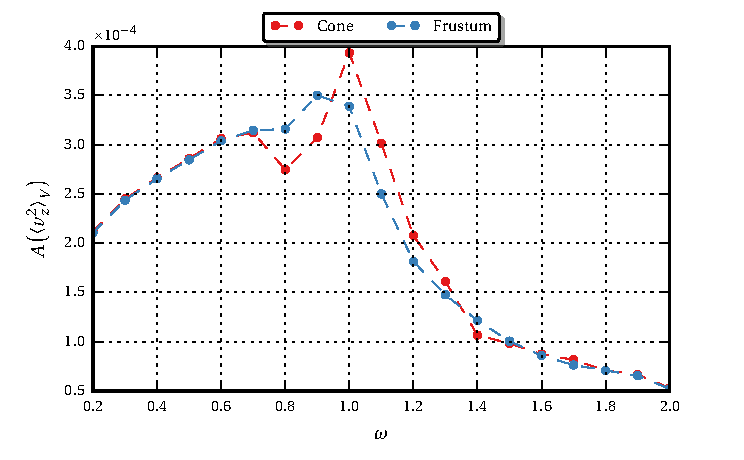
\includegraphics{gfx/cone/experiment/experiment.pdf}
  \caption{Amplitude $A\left(\left<v^2_z\right>_V\right)$ as a function of the libration frequency $\omega$,
            for the cone and the frustum.  \label{fig:cone_expseries} }
\end{figure}

The results of the simulations are shown in Fig. \ref{fig:cone_expseries}.
For both cases, the frustum and the cone, an increase in $A\left(\left<v^2_z\right>_V\right)$ can be observed.
From  about $2\cdot10^{-4}$ at $\omega=0.2$, to  $\approx 3.4\cdot10^{-4}$ for the cone and $\approx 4\cdot10^{-4}$ for the frustum,  at $\omega=1$.
From here on, the amplitude decreases to $\approx 5\cdot10^{-5}$ at $\omega=2$.
A difference between the two setups can be observed in the surrounding area of $\omega=1$.

For the frustum the increase of the amplitude is interrupted at $\omega=0.7$, a minimum can be observed at $\omega=0.8$, followed by
a peak at $\omega=1$. For the cone a minimum is not directly visible but it can be noted that the
amplitude does not increase as much at $\omega=0.7$ as for lower frequencies.\\
The maxima of the frustum ($\omega=1$) and cone ($\omega=0.9$) do not occur
at the same frequencies and have a difference of $0.5\cdot10^{-4}$ in amplitude.

However, it has to be considered, that due do the step width of $\Delta\omega = 0.1$ the exact position of the maxima is not apparent.
It appears that the expansion of the frustum to a cone leads to a frequency shift to the left.
Furthermore, it seems that the spectrum can be divided into two domains $0\leq\omega\leq1$ and $1 \leq \omega\leq 2$.
This result is not unexpected, since we choose the slope $\alpha$ of the cone such that $\omega_c=1$.

\clearpage

\begin{figure}[!pt]
  \centering
  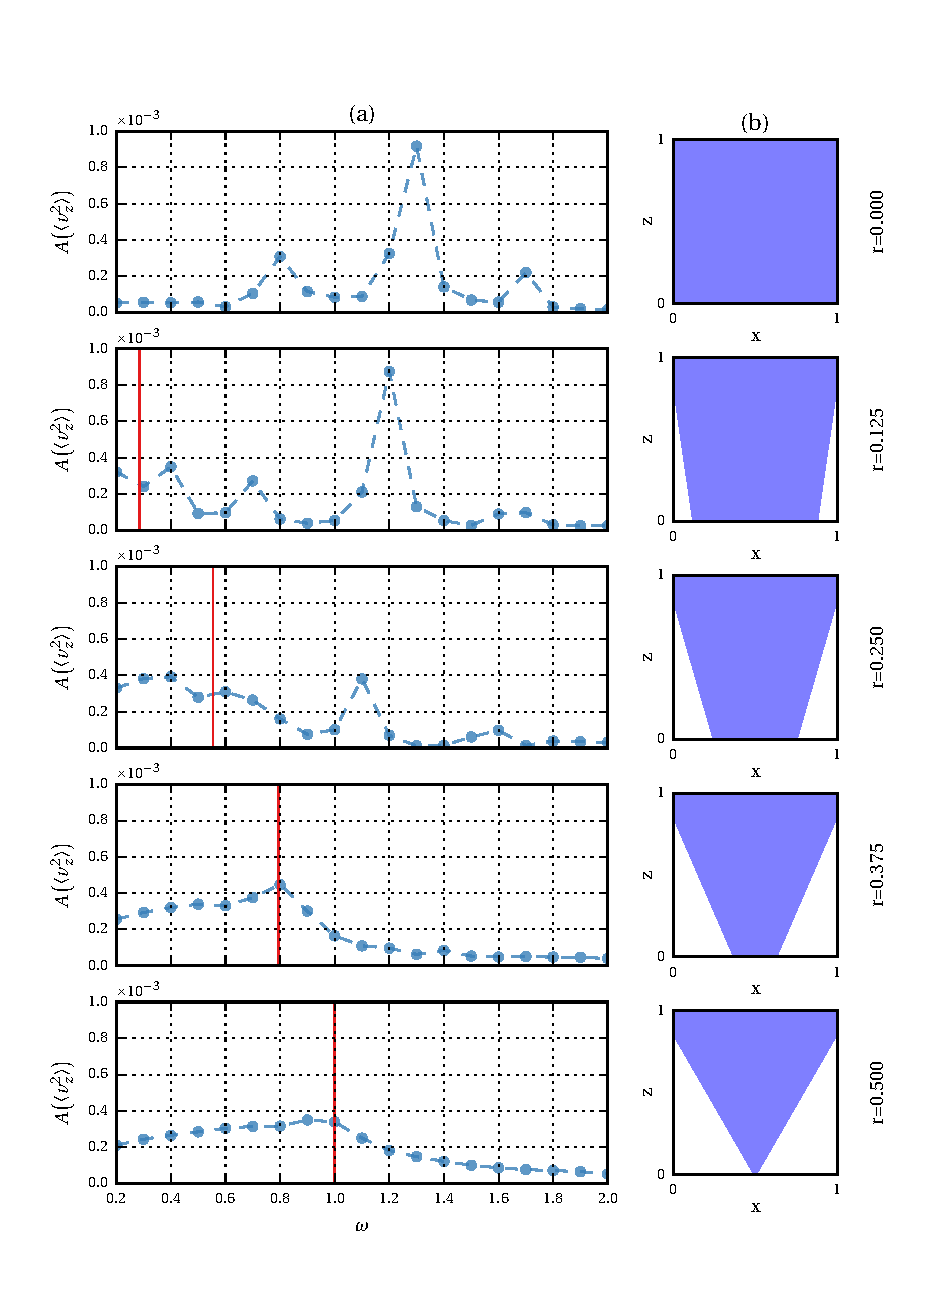
\includegraphics{gfx/cone/transition/transition.pdf}
  \caption{\label{fig:cone:transition}
      Amplitude $A\left(\left<v^2_z\right>_V\right)$ as a function of the libration frequency $\omega$,
      for the transition from a cylinder to a cone.
  }
\end{figure}

\clearpage
\subsection{Transition from a Cylinder to a Cone }

The results for the simulations are shown in Fig. \ref{fig:cone:transition}.
On the left side of the plot  the frequency spectrum is shown, the right side illustrates the geometry used.
The radius $r$ decreases from the top to the bottom.
For $r=0.5$  the inertial modes of a librating cylinder can be observed, which is in accordance
to the results of the librating  cylinder, wich we discussed in Sec. \ref{cone:sec:lib_cylinder}.
The result for $r=0$ is identical to the simulation of the cone from the previous section.

With a decrease of the radius a change in the position and amplitude of the
inertial modes is visible.

This pattern shall be exemplarily discussed  for the (2, 1) mode at $\omega=1.3$, where it is best visible.
For all other modes the transition results in a similar behavior.

The decrease of the radius leads to a shift to lower frequencies of the (2, 1) mode,
from $r=0.5$ to $r=0.375$ it is of the order $\Delta \omega=0.1$.
It can be noticed that during this shift, a damping of the mode occurs.
For $r=0.5$ the amplitude is about $9.2\cdot10^{-3}$, for $r=0.375$ it is
about $8.7\cdot10^{-3}$ and for $r=0.25$ we obtain $3.8\cdot10^{-3}$.
Whereas the first decrease of the radius does not significantly affect the amplitude,
the second decrease leads to a strong damping to less than half of the original value.
With a further decrease in $r$, the (2, 2) mode is annihilated.
For the (4, 1) mode, a slight increase of the amplitude at $r=0.125$ is still noticeable.
In addition this mode is stronger damped for $r=0.375$, in comparison to the (2, 1)-mode.

The vertical lines in Fig. \ref{fig:cone:transition} are set to the position $\omega=\omega_c$.
The area $\omega<\omega_c$ can again be associated with the frequency domain, where the wave propagation angle $\theta$ is larger than
the  slope of the cone $\alpha$, so that downward traveling waves propagate to the top after a reflection.
In can be noted that in this area the amplitudes increase, which is in accordance with the
results from the simulation of the experiment.

\clearpage


\subsection{Results of the Cone and Frustum with Different Offsets at the Top}
\subsubsection{Spectrum}

The results for this simulation are shown in Fig. \ref{fig:cone:finaltransition}.
On the left side of the plot  the frequency spectrum is shown, the right side illustrates the geometry used.
The height $h_+$ is in descending order, from top to bottom.
Each plot contains two spectra, one for the cone (green)  and the other one for the frustum (blue).
We begin with a qualitative description of the curves for the frustum.\\
At all heights $h_+$ several resonance modes can be observed. For the height ${h_+=0.25}$
the largest peaks occur in the spectrum, which are numerated here in decreasing order of the amplitude.
The largest peak M\RN{1} can be observed at a frequency $\omega=1.25$ and an amplitude of $5\cdot10^{-4}$.
The next resonances are: M\RN{2} at $\omega=0.9$, $A=3.7\cdot10^{-4}$, M\RN{3} at $\omega=0.5$,  $A=2.8\cdot10^{-4}$.
On the right side of the spectrum there are two possible small resonances at $\omega=1.7$ and $\omega=1.5$ (M\RN{4} and M\RN{5}).
For the case $h_+=0.5$  small additional resonances  M\RN{6} at $\omega=1.8$ and M\RN{7} at $\omega=0.55$ can be noticed,
the latter is embedded in the slope of the M\RN{3} peak.

Let us now consider the results of the cone.
Above the critical slope $\omega\geq\omega_c$, nearly all resonances are eliminated,
with two exceptions, the M\RN{6} and \textbf{O} peak for $h_+\geq0.375$.
The \textbf{O} peak can be associated with an M\RN{1}-mode for the cone.
For further discussions the minimum $\omega_{\text{min}}$ to the left of M\RN{6} is shown.

On the left side of the critical frequecy $\omega_c$, we can identify the M\RN{3}-peak
at the same frequency and same order as for the frustum. To the left side of this point, the spectrum for
the cone and the frustum are similar.
Furthermore at the position of peak M\RN{2} of the cone, we now see a slightly diminished peak M\RN{8}.
The maximum has the same position for $h_+=0.5$, but diverges slightly with a decrease of the height $h_+$.

For all peaks  it can be noted, that a lowering of the offset height $h_+$ results
into a shift towards higher frequencies. %This can be best seen when looking at the peaks M\RN{1} and M\RN{2}.
For a better overview, the changes in the amplitudes and shift in the frequencies are shown in
Fig. \ref{fig:cone:finalampmax}. %for the peaks M\RN{1}, M\RN{2}, M\RN{3} and M\RN{8}.
The amplitudes of the two peaks M\RN{1} and M\RN{2} have a maximum at $h_+= 0.25$. For the peak M\RN{3} and M\RN{8} the amplitude decreases almost linear.
From the second plot it can be noted, that with a decrease in the height $h_+$,
all peaks shift approximately linear to lower frequencies.

In order to give a better insight of the modal structures, the velocity profiles for the peaks M\RN{1}, M\RN{2} and M\RN{8}
are presented in Fig. \ref{fig:cone:finalmodesexp}, for different geometries .
For each setup the velocity profile is shown for two different timesteps. The offset $\Delta t^*$ is varied  for each geometry, in order to emphasize
the important flow properties.
For the peak M\RN{1} and M\RN{2} in the frustum, the velocity profile looks like a standing wave,
in contrast to the cone where a downward traveling wave can be observed for the peak M\RN{1} and M\RN{8}.


\begin{figure}[!pt]
  \centering
  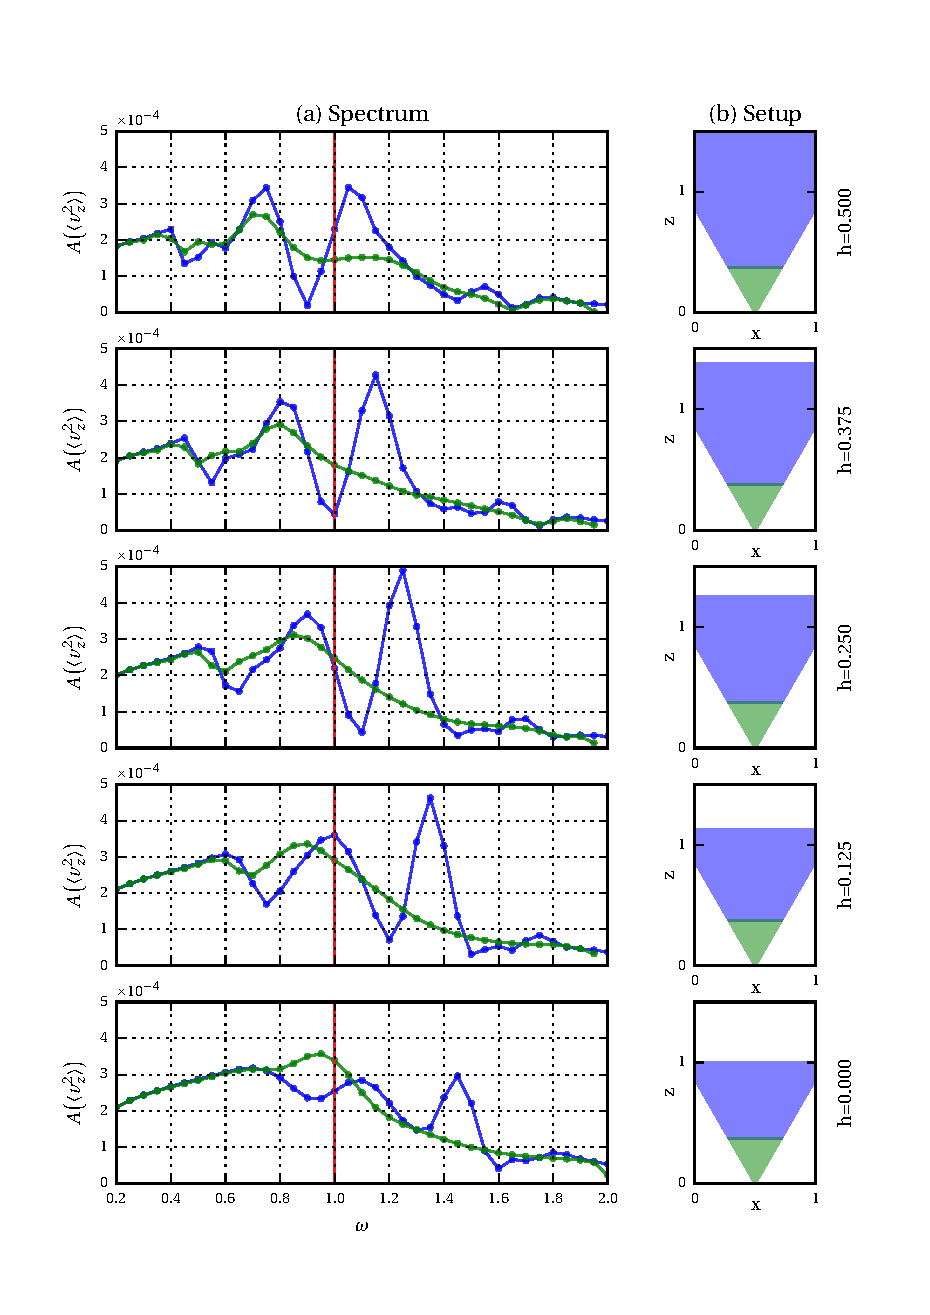
\includegraphics{gfx/cone/final/transition.pdf}
  \caption{
      \label{fig:cone:finaltransition}Amplitude $A\left(\left<v^2_z\right>_V\right)$ as a function of the libration frequency $\omega$,
      for the cone  and the frustum for different offsets $h_+$.
    }
\end{figure}
\clearpage

\begin{figure}[!tp]
  \centering
  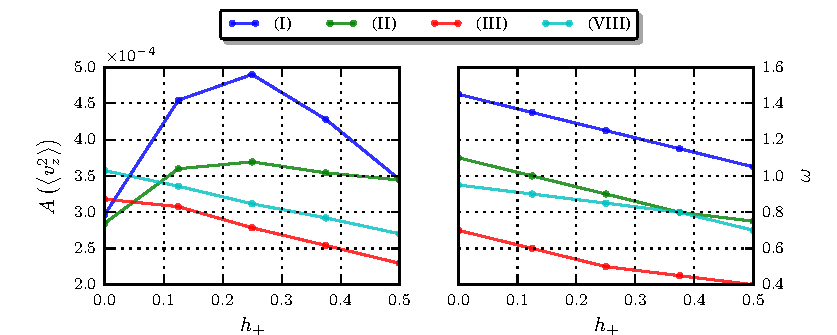
\includegraphics{gfx/cone/final/amp_pos.pdf}
  \caption{
      \label{fig:cone:finalampmax}Amplitude and frequency position of the resonances M\RN{1}, M\RN{2}, M\RN{3} and M\RN{8}
      for different offsets $h_+$.
    }
\end{figure}
\begin{figure}[!bp]
  \centering
  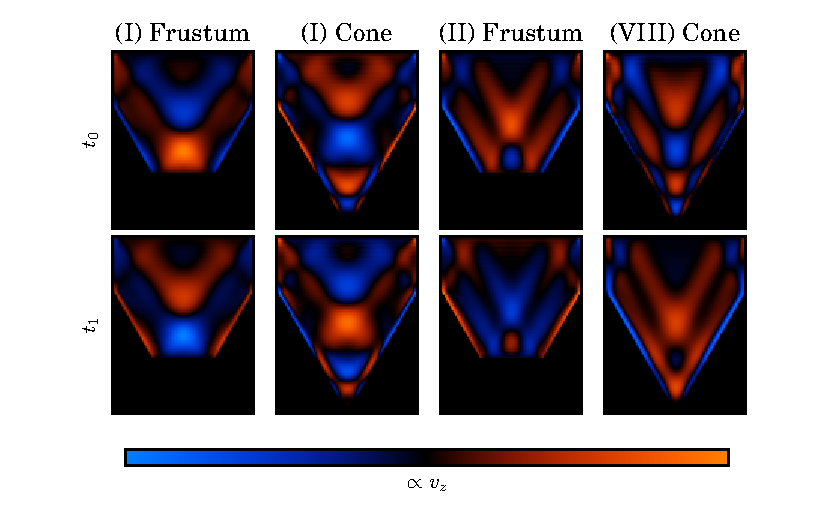
\includegraphics{gfx/cone/final/modes.pdf}
  \caption{
      \label{fig:cone:finalmodesexp}
      Velocity component $v_z$ in the $xz$ plane at y=\nicefrac{1}{2}.
       For the peaks M\RN{1}, M\RN{2} and M\RN{8} in the Cone or Frustum at $h_+=0.25$.
    }
\end{figure}
\clearpage

\subsubsection{Helicity}

The computed relative helicity shall be exemplarily discussed for  the case ${h_+=0.25}$.
For all other heights, frequency shifts and small changes in the amplitude can be observed,
that are not of importance for further discussions.
The results are shown in Fig. \ref{fig:cone:finalhelicity}.
For the computation, an inertial frame of reference was used.
Therefore an additional offset in the velocity,  given by
\begin{align}
    \vec{v} = \vec{v}|_{\text{rot.}} + \Omega(t) \times \vec{r} = \vec{v}|_{\text{rot.}} +
     \begin{pmatrix}
           -y (1 + \epsilon \sin(\omega t)) \\
           x ( 1 + \epsilon \sin(\omega t)) \\
           0\\
         \end{pmatrix}
\end{align}

has to be considered.
Furthermore the relative helicity was averaged over the time domain.
For both cases, the frustum and the cone, a positive helicity can be observed in the region $\omega<\omega_c$, which is
approximately $5\cdot 10^{-2}$.
At the critical slope $\omega=\omega_c$ the helicity decreases below zero and is of the order $10^{-1}$.
For $\omega>1.8$ the helicity is increasing slightly above zero to the order $10^{-3}$.
The differences, between the cone and the frustum are marginal.
However, it can be noted that the positions of the peaks M\RN{1}, M\RN{2} and M\RN{8},
correspond to an increase in the helicity.
Overall, it can be said that the computed relative helicity of the system is small in
comparison to the maximum value of 1.

\begin{figure}[!b]
  \centering
  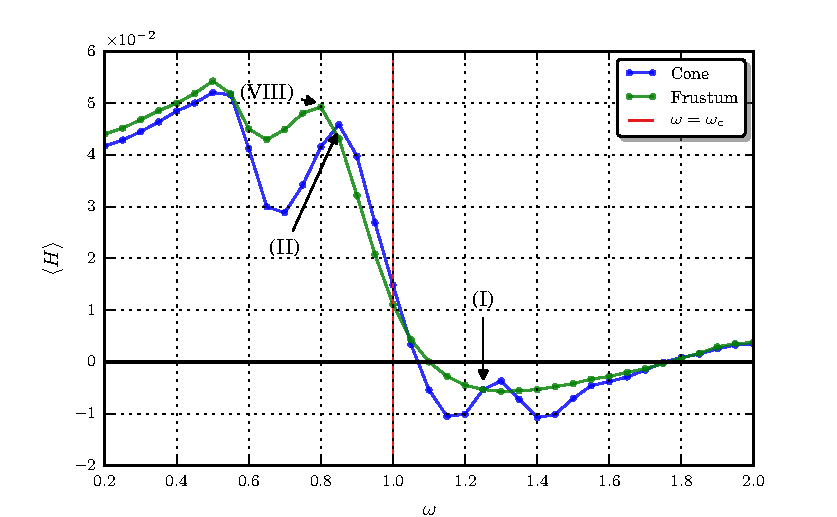
\includegraphics{gfx/cone/final/helicity.pdf}
  \caption{
      \label{fig:cone:finalhelicity}
      Relative helicity for $h_+=0.25$, of the cone and the frustum.
    }
\end{figure}

\clearpage

\begin{figure}[!b]
\centering
\begin{minipage}{.5\textwidth}
  \centering
  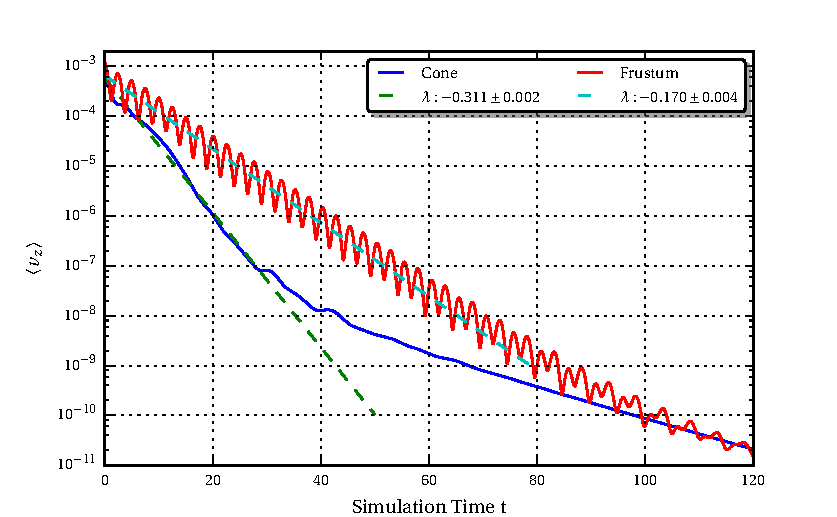
\includegraphics{gfx/cone/final/decay/decay_example.pdf}
  \caption{
      \label{fig:cone:finaldecayexample}
      Decay of the M\RN{1} peak in the frustum in comparison the cone.
    }
\end{minipage}%
\begin{minipage}{.5\textwidth}
  \centering
  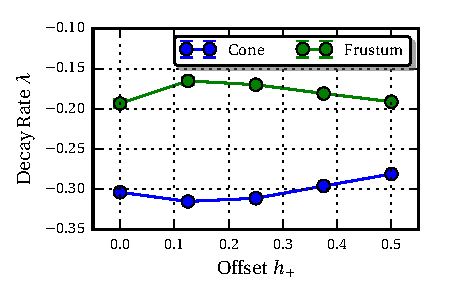
\includegraphics{gfx/cone/final/decay/fit_decay.pdf}
  \caption{
      \label{fig:cone:finaldecayfit}
      Interpolation of the decay rate $\lambda$ for different heights $h_+$.
    }
\end{minipage}
\end{figure}

\begin{figure}[!b]
  \centering
  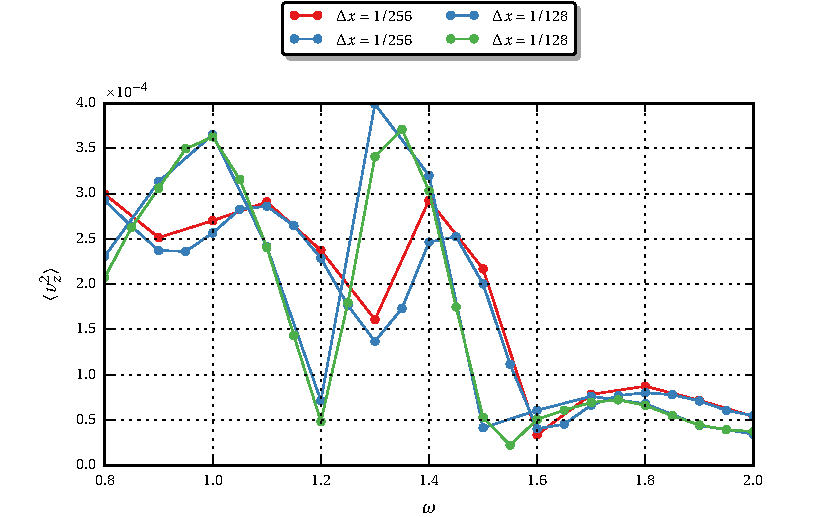
\includegraphics{gfx/cone/final/hd_comparison.pdf}
  \caption{
      \label{fig:cone:finalhdcomp}
      Comparsion of the results for the frustum to the same simulation with higher resolution.
    }
\end{figure}
\clearpage

\subsubsection{Decay Rates}

The simulation of the decay of inertial waves was performed for the peak M\RN{1} in the frustum,
for all heights $h_+$.
This coice is motivated by the position of M\RN{1} which is above $\omega_c$ for all heights.
Hence, the expectation is a fast decay into the apex for the cone and a slower decay for the frustum.
As a comparison the same frequencies were used for a simulation of the decay in the cone.
Fig. \ref{fig:cone:finaldecayexample} shows the decay exemplarily,
for $\omega=1.25$ and $h_+=0.25$ on a semi-log plot.

For both geometries there are two different decay rates observable.
For the frustum the first decay takes place in the time interval $t\leq 100$,
followed by a slow decay for $t>100$.
The cone shows a faster decay in the interval $ t\leq 30$, followed by a slow decay for $t>30$.
It can be noted that the energy in the cone decays faster until $t\approx100$, after this time
both decay rates are  equal.  In contrast to the cone, the decay of the frustum  is superimposed by an oscillation.

Fig. \ref{fig:cone:finaldecayfit} shows the interpolated values of the decay rate for different
heights $h_+$.  The time interval for the interpolation was set to $0 \leq t \leq 25$.
The decay rate of the cone is about $1.5-2$ times as large than the decay rate for the frustum.

Finally in Fig. \ref{fig:cone:decayphaseexample}, the velocity profile for different times, during the decay in
the frustum is shown.
It can be seen that as time passes, the wave is traveling into the apex of the cone.
A profile for the frustum is not shown here, but it should be mentioned that in this case reflections to the top occur
and the decay is homogeneous over the fluid domain.

\begin{figure}[!b]
  \centering
  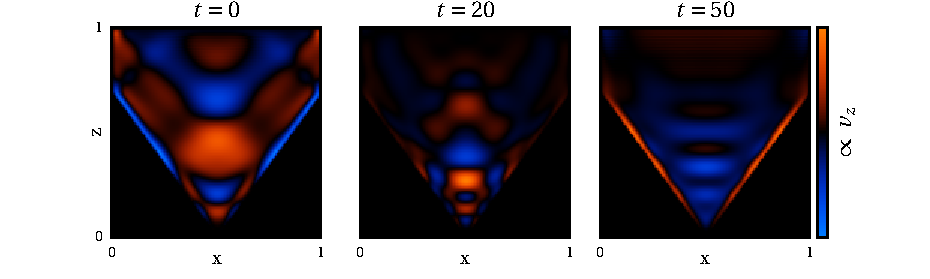
\includegraphics{gfx/cone/final/decay/phase_decay.pdf}
  \caption{
      \label{fig:cone:decayphaseexample}
        Velocity profile for the decay in the cone for different times, for $h_+=0.25$ and $\omega=1.24$.
    }
\end{figure}

\subsubsection{Comparison to a Higher Resolution}

A part of the simulations was repeated with a spatial discretization of $\Delta x= \nicefrac{1}{256}$.
Since the computation time at this resolution is expensive, the frequency was limited
to the interval $0.8\leq\omega\leq2$ with a stepsize of $\Delta \omega = 0.1$ and the heights
$h_+\in\{0.0, 0.125\}$.
The results in comparison to the lower resolution are shown in Fig. \ref{fig:cone:finalhdcomp}.
All peaks in the spectrum for the high resolution are in accordance with the previous computations.
It can be noted that the higher resolution spectra are slightly shifted to the top.
Furthermore it shall be mentioned that numerical oscillations, like for the cyinder
(see Fig. \ref{cone:cyl_oscillations}) are still present.
The amplitude of these oscillations is about half the size in comparsion to the oscillations for
a low resolution with $\Delta x = \nicefrac{1}{128}$.

\clearpage

\section{Discussion}
\subsection{Setup from the Experiment}
\label{cone:discussion_experiment}

For $\omega < \omega_c$ the results for both setups are similar.
A possible explanation is that in this domain the cone tip does not act as an attractor.
An inertial wave propagates to the top after a reflection on the side of the cone.
Hence, for both setups a similar spectrum exists.

The differences occur when $\omega$ reaches the critical frequency $\omega = \omega_c$. In this scenario, an inertial wave emitted from the
top edge, traverses directly into the apex of the cone, or is reflected slightly at the bottom plate of the frustum.
As a result we see the slight increase in the amplitude for the frustum.

For $\omega > \omega_c$ further resonances in the spectrum of the frustum should be observable,
since the bottom plate enables the reflection of inertial waves.
The similar decay of the amplitude for both geometries refutes this assumption.
Neither the experiment \citep{Beardsley1970} nor the theoretical description by \citep{Greenspan1990}
are in accordance with the results of the simulation.

An explanation could be given by the fact that a different Ekman number ($\Ekman = 10^{-4}$), was used for the simulations,
while the width of the envelope of an inertial wave ray can be estimated to $\Ekman^{\nicefrac{1}{3}}\approx 0.046$, according to \citep{Tilgner2000}.
The experiment used an Ekman number of $\Ekman = 10^{-5}$, resulting in a  width of $\Ekman^{\nicefrac{1}{3}}\approx 0.022$.
As a consequence, the width of an inertial wave ray is around twice the size as in the experiment.
It can be assumed that a wave reflecting on the bottom of the frustum
is stronger damped as in the experiment.
The bottom plate of the frustum is too narrow to support an efficient reflection
of inertial waves, due to frictional losses.\\

\clearpage

\subsection{Transition from a Cylinder to a Cone}
\label{cone:discussion_transition}

The objective of this simulation was to study the previous assumption,
by varying the radius of the bottom of the frustum and investigate the influence
on the reflection of inertial waves.

The simulation shows that the transition from the cylinder
to the frustum results in a shift of the modes.
Furthermore it can be seen that the all modes are damped with a decrease of the bottom gap width.
An explanation for the shift can be given by having a look at the inertial mode structure,
for different radii as shown in Fig. \ref{fig:cone:phase}, for the (2, 1) mode.\\
For $r=0.5$ we have an inertial mode, which is symmetric to the plane $z=h/2$.
In this plane, the waves excited from the bottom and top of the cylinder, annihilate each other to a wave node.
An decrease of the radius breaks the vertical symmetry of the inertial mode.
As a result only a distorted version of the mode can exist, where the center of the wave node
is shifted downwards.

\begin{figure}[!b]
  \centering
  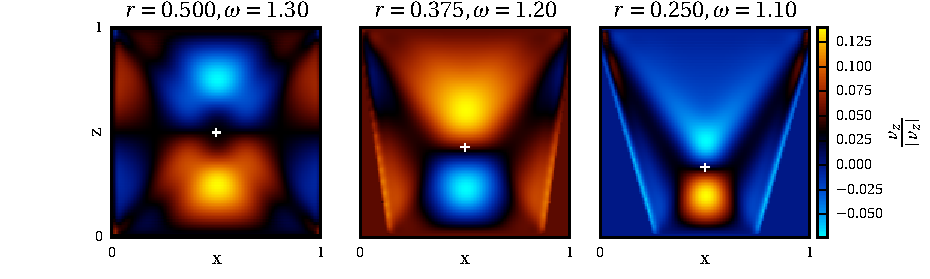
\includegraphics{gfx/cone/transition/phase.pdf}
  \caption{\label{fig:cone:phase}
    Inertial mode structure for the (2,1) Mode from the cylinder at different radii on the bottom of the frustum.
    The white points mark the center of the wave node, computed with Eq.  \ref{cone:wavenodeeqn}.
  }
\end{figure}

The attempt was made to obtain the new position of the center,
by computing the intersection of the diagonals, from the top to the bottom edges of the frustum.
The resulting center height is given by

\begin{align}
\label{cone:wavenodeeqn}
c  = r \frac{h}{r+\nicefrac{l_x}{2}}
\end{align}

The resulting points are in a good agreement, as the marked position in Fig. \ref{fig:cone:phase} show.
For the same inertial mode the propagation angle $\theta$ has to be
increased for it to exist in the narrower shape.

This is equivalent to a shift to a lower libration frequency.
For $r \rightarrow 0$ the center position converges against zero. Hence, the mode cannot exist in this state.

\clearpage

\subsection{Librating Cone and Frustum with Different Offsets on Top}

\subsubsection{Motivation}

For the simulations which have been carried out to this point in this thesis,
the influence of the offset on top of the cone has been left out from any discussion.
As we saw, this offset has an influence on inertial wave propagation.
In particular for the intervall $\omega<\omega_c$, where  downward traveling waves are
reflected upwards.
In the case where the offset is set to zero, the corners of the cone act as an attractor.
For small gap sizes it could be possible that an inertial wave will be damped,
which is in accordance with the previous results.
This motivates a simulation series with different offsets.
The simulation of the transition from a cylinder to a cone showed
that a damping acts on an inertial wave when reflecting at the bottom,
which  depends on the radius of the bottom gap.
This motivates the use of a larger radius at the bottom in comparison to the experiment.

\subsubsection{Spectrum}

For both scenarios, the cone and the frustum, resonances can be seen.
The observation of the velocity profile for these resonances indicates,
that the peak M\RN{1} and M\RN{2} are inertial modes in the frustum.
One assumption was that the resonance M\RN{8} is related to the M\RN{2} mode.
However, the velocity profile of M\RN{8} indicates a downward traveling wave.
Since it is located below the critical slope $\omega < \omega_c$, the cone apex
should not act as an attractor, which is in contrast to this observation.
The propagation angle for M\RN{8} is about $65^\circ$.
For this value a wave ray originating from the upper edges of the cone travels directly
into the cone apex.
A possible explanation is that such a wave is not reflected due to damping effects in
the apex of the cone. As a result, a downward traveling wave is observed.
However, with this approach we are still not able to explain the resonance of the M\RN{8} peak
in the spectrum.

The shift of the resonance peaks is a result from the change in the geometry.
In analogy to the discussion in Sec. \label{cone:discussion_transition},
 we assume that with a change of the offset on top,
a possible inertial mode can only exist in an distorted state.
Therefore the propagation angle $\theta$ has to change,
which is equivalent to a shift in the frequency domain.\\
We were not able to find a reasonable explanation for the change in the amplitudes.
The assumption was that for $h_+=0$ the damping due to the small corners at the top
would diminish the amplitudes the strongest.
For the inertial modes M\RN{1} and M\RN{2} an increase of the amplitude is observed until $h_+=0.25$,
which is in accordance with the assumption.
But the decrease for $h_+>0.25$ is difficult to explain.
Even more confusing are  the peaks M\RN{3} and M\RN{8} where a decrease in the amplitude
can be observed.

\begin{figure}[!t]
  \begin{minipage}[c]{0.4\textwidth}
      \centering
      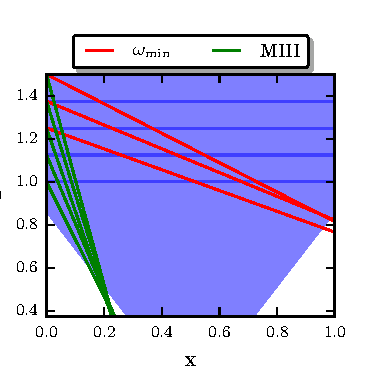
\includegraphics{gfx/cone/discussion/corners.pdf}
  \end{minipage}
  \hfill
  \begin{minipage}[c]{0.5\textwidth}
      \caption{\label{fig:conediscuss:corners}
        Wave paths from the upper edges of the cone,
        for a wave ray with a frequency at the position $\omega_{\text{min}}$ (red) and
        for a wave ray with the frequency at the position of peak (\RN{3}) (green),
            for different heigths $h_+$.
      }
  \end{minipage}
\end{figure}


%The next point in this discussion is the M\RN{6} mode.

For the cone geometry the M\RN{6} resonance is still apparent.
The assumption that this resonance is an inertial mode,
violates the argument that the apex of the cone acts as
an attractor.
A possible explanation is given in Fig. \ref{fig:conediscuss:corners}.
The plot shows the wave path from an upper edge of the cone, for the frequency $\omega_{\text{min}}$.
With an increase in the frequency the propagation angle decreases.
For $\omega<\omega_{\text{min}}$ the wave is reflected on the slope of the cone.
For $\omega>\omega_{\text{min}}$ the reflection is above the slope on the walls resulting from the offset $O$.
The assumption is that the reflection on the slope of the cone creates more dissipation.
This is due to the Direct-Forcing method, which creates a more pixelized border on the slope,
in comparison to the side walls on top of the cone.
As a result the energy and therefore the amplitude increases,
when the wave ray is passing the corner to the top.
With this argumentation it is still not possible to explain the slight increase \textbf{O}.


A similar idea can be applied to the left side of the peak \RN{3} (see Fig. \ref{fig:conediscuss:corners}).
For $\omega<\omega(\text{M\RN{3}})$ the wave is reflected off the slope of the cone.
for  $\omega>\omega(\text{M\RN{3}})$ the reflection moves to the bottom plate of the frustum,
or remains on the slope in case of the cone.
This could explain why for   $\omega<\omega(\text{M\RN{3}})$  the spectra look identical,
since the wave ray does not see the difference between the cone and the frustum.
This argumentation is furthermore consistent with the results from the first simulation
(see discussion Sec. \ref{cone:discussion_experiment}).
It has to be concerned that these are of course theoretical assumptions and a wave ray is not only emitted at the
upper edges of the cone.\\ (TODO: EXPLANATION CHARACTERIST SURFACES)

As a last point of the discussion of the spectrum, we go back to the M\RN{1} inertial mode.
The results of the simulations show that an inertial mode exists for the frustum.
When taking away the bottom plate the inertial mode is not apparent instead
a downward traveling wave into the apex can be observed.
This results is in excellent agreement with the theoretical ideas and the experiment we introduced in Sec.
\ref{cone:theorie_exp}, \ref{cone:theorie_theo}.
\clearpage
\subsubsection{Helicity}

The objectve behind the computation of the helicity was to see if this system could be used
for further simulations, concerning MHD-equations and the generation of a dynamo.
The results show that the total helicity of the system is not zero in contrast to the cylinder.
An explanation therefore can be given by the asymmetry of the system in $z$-direction.(MORE DETAILS?)
The frequency spectrum of the relative helicity of the  system can be separated into two different regions.
For $\omega<\omega_c$ the largest helicity of order $5\cdot10^{-2}$ is observable.
It can be said that this value is too small to be of interest for further researches.
\footnote{Private Communication A.Tilgner}


\subsubsection{Decay Rates}

The computed decay rates show that an inertial mode in the frustum has a slower decay
than the equivalent case in the cone.
The velocity profiles furthermore show that in the frustum the inertial mode decays homogenously over the whole domain.
In case of the cone an inertial wave travels down into the cone, where it decays.
Those results furthermore demonstrate that the apex of the cone is acting as an attractor.
With that in mind it can be said that the system could be interesting for further researches,
for example the study of the decay of turbulences in the apex of the cone.

\subsubsection{Higher Resolution Simulation}

The resulting frequency spectra for the higher resolutions show,
that the default resolution of ${\Delta x = \nicefrac{1}{128}}$ yields
qualitative comparable results, since the overall appearance of the resonance spectrum
is equal.
For a better comparison it could be interesting to repeat the simulations with a
higher resolution in the frequency stepping and a smaller Ekman number.
Furthermore the resulting velocity profiles support the assumption
that the numerical oscillations are based on the Peclet criterion.(MORE DETAILS?)
Since the oscillations are small with respect to the physical solution and not
growing over time, the error is acceptable for the moment.
However a simulation of smaller Ekman numbers could be problematic.
\clearpage

\section{Summary}

\subsection{Librating Cylinder}


In the first part of the chapter we reviewed the simulation of a librating cylinder.
The simulation was performed as a validation test case for the cone,
since for this system more literature is available for comparison.
The obtained frequency spectra revealed three inertial modes,
which are in good agreement with the theoretical results from \citep{Greenspan1990},  and the  numerical results from \citep{Sauret2012}.
Furthermore it could be shown that all immersed boundary methods were able to reproduce these modes.
The only exception is the interpolation method, which is numerically unstable.
This is a little bit of a disappointing result, since this methods tends to contain
the smallest numerical error.
Finally, the results show an error regarding the numerical implementation.
For all test cases numerical oscillations could be observed which are related to the
large Peclet number of the system.
These oscillations are not directly an issue, since a growth of the error amplitude over time could not be observed.
Beside that, it has to be considered that the error is small in comparison to the physical solution of the system.

\subsection{Librating Cone}

In the second part of the chapter different simulations of
a librating cone and a librating frustum were reviewed.
The first simulation was oriented towards the experimental setup described in \citep{Beardsley1970}.
However, the results  were not agreement with the experiment.
The assumption was made that the difference is based on the  stronger damping of inertial waves,
due to the use of a larger Ekman number.
In the second simulation the influence of the bottom radius of the frustum was varied
to test the influence on the ability of inertial wave reflection.
It could be shown that a smaller radius leads to a damping of an inertial mode and that the frequency
shift is related to a distortion of the inertial wave geometry.

In the last simulation series  the offset on top of the cone was varied, in order to test the influence on
inertial wave propagation. Secondly, the gap radius was set to a large value in contrast to the experiment,
to enable a better reflection in accordance with results from previous simulations.
The results  show that the offset on top affects the position and the amplitude of the resonances
found in the frequency spectrum.
The simulation furthermore showed that inertial modes in the cone exist.
More important is the result that the replacement of the frustum with a cone annihilates possible
inertial modes for $\omega > \omega_c$.
Waves are reflected downwards into the apex, which is in good agreement with the
theoretical discussion of \citep{Greenspan1969} and the experiment by \citep{Beardsley1970}.

